%!TEX root =../MacbethThesis.tex
\acresetall
\chapter{A Rule-Engine for Electronic Institutions}\label{ch:droolseinst}

\lettrine[lines=3]{E}{lectronic} Institutions have been identified as a powerful
tool for maintaining order and cooperation in `open' multi-agent
systems~\citep{Esteva2001,Artikis2009}. Taking lessons from the development of
institutions (defined as sets of rules which define what is permitted and
forbidden within a given context~\citep{Ostrom1990,North1990}) in human social and
organisational systems, they aim to regulate interactions as norms---specifying
expectations of behaviour---or concrete rules to say what is required and
forbidden.

This set of rules has been given other names in the context of multi-agent and
agent-based systems. \citet{Artikis2009} specify ``norm-governed'' systems,
however these `norms' are analogous to institutional rules, in that they are
social constraints on the actions of agents within an arena. Similarly, an
institutional rule can be called a `policy', as often seen in network
management ~\citep{Sloman1999}. In all cases, the institution is assigning
some form of institutionalised power, permission and/or
obligation (cf.~\citet{Jones1996}) for agents to perform certain actions (and it has
been argued that this kind of assignment is essential to properly specify a system which extends beyond purely physical state~\citep{Artikis2009a}).
In an open system any agent could perform any action (within its physical
capabilities). An electronic institution used in the context is able to
distinguish between actions which should and should not cause a change in
institutional state, and actions which are allowed and forbidden.

% \citet{Artikis2009} specify what they call both ``open agent societies'' and
% ``norm-governed computational societies'' as systems with unpredictable,
% heterogeneous agents to whom we wish to foster normality and compliance in order
% to achieve desirable system goals. The framework defines 
%  to apply social constraints through
% institutionalised power, permission and obligation~\citep{Jones1996}, as well as
% sanctions and enforcement policies. 

% \lettrine[lines=3]{E}lectronic Institutions are a useful tool for implementing
% governance in agent-based systems~\citep{Esteva2001}. Institutions are defined
% as sets of rules which define what is permitted and forbidden within a given
% context~\citep{Ostrom1990}. Institutions are also built with the capability to
% change themselves, giving self-adaptive properties~\citep{North1990}. The
% implementation of electronic institutions, therefore, has focused on the use of
% rule-engines and action languages~\citep{Artikis2012a,Arcos2005,Garcia-Camino2009}.

% When specifying an electronic institution we are defining rules within some
% arena which determine who has \emph{institutionalised power}, \emph{permission}
% and \emph{obligation} to perform certain actions~\citep{Jones1996}. In an open
% system any agent could perform any action (within its physical capabilities). An
% electronic institution used in the context is able to distinguish between
% actions which should and should not cause a change in institutional state, and
% actions which are allowed and forbidden.

A institution may also make agents aware of when they have the power,
permission or obligation to do an action. This aids in the planning of actions,
so that agents do not waste energy with ineffectual actions, or worse, forbidden
actions which may lead to sanctions. For example, most governments will notify
their citizens of the time window in which going to ones local polling station
and marking a cross on a piece of paper will count as an election vote. Outside 
of this window this action has no effect.

Thus, an implementation of an electronic institution should be an executable
specification which, firstly, holds some state of the institution, though which
powers, permissions and obligations can be deduced, secondly, defines how
actions may change the state of the institution at a given time, and, finally,
allows agents to query whether they are empowered, permitted or obliged to perform
any given action.

Furthermore, in human organisations, certain useful procedures have been
formalised and specified in such a way that they can be reused in institutions
as a tool for certain tasks. For example, \ac{RONR}~\citep{Robert2011} is a
specification of a parliamentary authority for organisations. Organisations
can take this specification and update their institutional rules accordingly
to incorporate this robust protocol. The aim of electronic institutions is to
provide such tools for open, agent-based systems, and work has been done on
specifying various protocols, include the a voting protcol from the aforementioned
\ac{RONR}~\citep{Pitt2005a}, floor control
protocols~\citep{Artikis2004,Artikis2009b}, monitoring and sanctioning
procedures~\citep{Pitt2012c}, argumentation~\citep{Artikis2003} and auctions~
\citep{Rodriguez1997}. However, there has yet to emerge an integrated tool
providing a suite of these protocols for use by institution designers.

We are concerned with how to implement electronic institutions for both
simulated applications and real-time system monitoring. This implementation
should therefore meet the following requirements:
\begin{itemize}
\item Fast-enough for real-time systems;
\item Expressive, such that complex rules and relationships can be implemented;
\item Readable, such that the behaviour is apparent from the specification;
\item Modular, such that institutions can be built up from the composition of smaller modules.
\end{itemize}

In this chapter we investigate the specification and execution of electronic
institutions. We review languages for specification of institutional rules.
Taking the Event Calculus as an example, we assess its use for the execution of
voting as per Robert's Rules of Order. My profiling the performance in this representative task, we show how performance can be drastically
improved using a naive rule-based implementation of the Event Calculus. Finally,
we argue that a business-rule engine has the necessary features to implement
electronic institutions, and show how Event Calculus specifications can be
translated to the JBoss Drools rule engine, using the \ac{RONR} example. 

% Distinction between physical and other capabilities (Artikis2009)

\section{Defining Electronic Institutions}\label{sec:instdefn}

To this point we have yet to formally define what we mean by an Electronic
Insitution, beyond saying that they are an instantiation of what economists
define as an Institution, but in a computational domain. \citet{North1990}
defines Institutions thusly: 

\begin{quote}
``Institutions are the rules of the
game in a society or, more formally, are the humanly devised constraints that
shape human interaction.''~\citep[p.3]{North1990}
\end{quote}

Despite this definition, institutions are often confused and conflated with
organisations. This is partly because many organisations are called
`institutions', for example an `academic institution' refers to the
organisation, not the rules. It is also because it is within an organisation
that institutions function:

\begin{quote}
``A crucial distinction \ldots\ is made between institutions and organizations.
\ldots\ Conceptually, what must be clearly differentiated are the rules from the
players.''~\citep[p.4]{North1990}
\end{quote}

Therefore, if we consider an institution as a set of rules governing the
interactions, and constraints thereon, between humans within a society, then
we can consider \emph{electronic} institutions as rules governing interactions
between actors within a computational domain. Note, this does not mean that all
of the actors are computational agents---socio--technical systems require
institutions which can be applied uniformly to both human and computational
actors. The distinction between a human and electronic institution is that the
latter is specified and executed in a computational domain.

\citet{Esteva2001} specify electronic institutions with a similar definition,
also derived from the definition of \citet{North1990}. Their specification allows
the institution to dictate how and when interactions occur via a
\emph{dialogic framework} (a common language of communication) and
\emph{scenes}, which define subgroups where dialogues occur. These
\emph{scenes} are then linked together via a \emph{performative structure},
and \emph{normative rules} describe when actions are obligatory and/or
forbidden.

The concept of electronic institutions appears frequently, however often not
named as such, in open agent systems and normative systems.
\citet{Artikis2009a} survey the specification of these systems, including the
aforementioned framework of \citet{Esteva2001}, and in all cases some kind of
rule or constraint set is used to establish norms or desired interaction
patterns. In \emph{Artificial Social Systems}~\citep{Moses1995} a set of
restrictions on agents' behaviour, called \emph{social laws}, are specified.
\emph{Enterprise Modelling}~\citep{Fox1995} uses constraints on members of an
organisation, including normative relations such as obligation, authority and
empowerment. Finally, \emph{commitment protocols}~\citep{Chopra2006} are another method which has
been used to express normative relations between agents and establish order to
an open system.

However, \citet{Artikis2009a} argue that all four approaches fall short on their
specification of institutionalised power, particularly of `empowerment'; and their
handling of non-physical, or `institutional' facts and actions. \citet{Jones1996}
state the utility of empowerment as part of a normative framework, and it is
lacking in each of the surveyed approaches. To address this, \citet{Artikis2009}
give a specification of social constraints which expresses: 
\begin{itemize}
\item physical capabilities;
\item institutionalised powers;
\item permissions, prohibitions and obligations; 
\item and sanctions and enforcement polices to deal with forbidden actions.
\end{itemize}

This specification represents a superset of an electronic institution
specification. Physical capabilities are obviously outside of the scope of the
electronic institution, being a social construct it cannot constrain what
agents do physically. On the other hand, institutionalised powers and
permissions, prohibitions and obligations are obviously within the
institution. We argue that the final set of constraints---sanctions and
enforcement policies---are actually a feature which the institution \emph{may}
provide, but not part of its definition.

\citet{North1990} also states that a defining feature of human institutions is
that they can be changed by the organisations which use them. This
institutional change allows the organisation to adapt to changing conditions
and/or optimise inefficiencies (although it can also make things worse), and as such,
is an important property to translate. \citet{Artikis2012a} extend their
specification of open agent systems to enable the specification, which
contains the institutional rules, to change over time as a result of agent's
actions.

Therefore, we define an Electronic Institution as a set of executable
rules which specify:

\begin{itemize}
\item Institutionalised powers, and how they change, over time
and through the actions of agents. 
\item Permissions, prohibitions and obligations of
the agents.
\item How rules can be changed.
\end{itemize}

\section{Executable Specification of Electronic Institutions}

As we have defined that for an institution to be electronic it must be
executable, we now re-visit electronic institution specifications, and
particularly, their operationalisation. 

Work on specification of constraints, or norms, for multi-agent
systems often focuses on the use of logics for specification. Logical
specifications have the advantage of enabling model checking and formal proofs
of validity. Logics typically also support deductive, adductive and inductive
reasoning:

\begin{itemize}
\item Deductive tasks (also called \emph{projection} or
\emph{prediction}) determine ``what is true when'', given ``what happens
when'' and ``what actions do''. 
\item Abductive tasks (also called
\emph{postdiction} or \emph{planning}) determine ``what happens when'', given
``what actions do'' and ``what is true when''. 
\item Inductive tasks
(\emph{learning} or \emph{theory formation}) determine ``what actions do''
given ``what is true when'' and ``what happens when''. 
\end{itemize}

Action languages are a
particularly popular specification language, due to their incorporation of
state while maintaining logical semantics and satisfiability checking.
However, we often see performance issues when scaling executable
specifications of this type, as we will see later in this chapter.

\citet{Arcos2005} specify rules and constraints in first-order and deontic
logic, however these must then be translated into custom declarative
specification language for their \emph{ISLANDER}~\citep{Esteva2002} tool,
which can then verify the specification. This specification can be executed
within their \emph{AMELI} platform. \citet{Aldewereld2006} also proposes the
translation of logic, this time into constraints. In their \emph{HarmonIA}
framework, \citet{Vazquez-Salceda2003} go further, proposing four levels of
translation, starting with high level abstractions of statutes and norms which
eventually are translated into computationally efficient procedures.

\citet{Chopra2006} use the action language \emph{C+}~\citep{Giunchiglia2004}
to specify their commitment protocols. \citet{Artikis2009} also use this
language in their specification. This language allows the representation of
the properties of actions, including those with conditional and indirect
effects. There is also an implementation of the \emph{C+} language, the Causal
Calculator\footnote{http://www.cs.utexas.edu/users/tag/ccalc}, which
translates \emph{C+} action descriptions into propositional logic then allows
querying of the compiled system. Queries can perform deductive and abductive
tasks given both partial or complete information.

In addition to \emph{C+}, \citet{Artikis2009} employ the \ac{EC}. Like
\emph{C+} it is a formalism for representing and reasoning about actions and
their effects in a logic programming framework. It has an implementation in
Prolog which is capable of deduction, abduction and induction.

Finally, \citet{Cliffe2006} use answer set programs~\citep{Baral2003} to model
institutions, using a specification language semantically very similar to the
\ac{EC}. They argue that their formalisation has several advantages over both
\ac{EC} and \emph{C+}, largely related to simplifying the execution of
specifications from an algorithmic perspective.

We chose the \ac{EC} for our work for several reasons. It is easy-to-use and
intuitive. As Prolog compiles specifications very quickly, one can very
quickly test implementations, avoiding some of the longer development cycles
we introduced above. Furthermore, the majority of the protocols and
specifications we wish to use already have implementations in \ac{EC}.
Therefore, it appears, to us, a good starting point for a library of tools for
electronic institutions.

% There are several methods of specifying electronic institutions. In their
% survey, \citet{Artikis2009a} cover four methods given for open agent systems,
% one of which being `Electronic Institutions', as defined by \citet{Esteva2001}.
% As we have mentioned, our definition of electronic institutions is analogous to
% that which \citet{Artikis2009} give for a ``norm-governed society'' or ``open
% agent society'', characterised by institutional constraints and institutionalised
% power. Thus we start by assessing these four methods for, firstly, specification
% of electronic institutions, and secondly, how these specifications can be
% executed.

% \citet{Rodriguez-Aguilar2002} define an electronic institution with agents
% occupying roles who interact via speech acts. The institution specifies a `
% dialogical framework'---a common language for communication---for interactions.
% These interactions occur in `scenes', which encapsulate localised interactions
% in the system. The inter-connection of scenes forms a `performative structure'
% which describes the relationships between scenes. Finally, normative rules
% capture the obligations and prohibitions of agents.

% % Speech act/dialogical based (Aldewereld2007)
% Similarly, \citet{Aldewereld2006} define norms in terms of dialogues of speech
% acts, expressed in first-order logic. These expressions are then translated into
% declarative constraints to enable operationalisation of the norms. \citet{Fox1995}
% express organisational rules, including `permission', `right' and `authority',
% in a dialect of the Situation Calculus~\citep{Pinto1993}.

% The Gaia methodology~\citep{Wooldridge2000}, a general agent-oriented design
% method, has been extended to incorporate organisational rules~\citep{Zambonelli2003},
% however 

% HarmonIA - 4 level normative system (Vazquez-Salceda2003)
% The Harmon\emph{IA} framework, proposed by \citet{Vazquez-Salceda2003},

% Electronic institution vs Normative system
% Executable spec vs formal spec
% Features: abduction, deduction, provability
% Casual calculator: Prediction, planning, postdiction.
% Model checking - cannot be fordidden and obliged at the same time.

\section{The Problem with the Event Calculus}\label{sec:ecperf}

The \acl{EC}\footnote{We gave a brief primer on the \ac{EC} and its predicates in \autoref{sec:ecprimer}. A more detailed introduction to the concepts can be found in \citet{Shanahan1999}.} is a good formalism for executable specification of electronic
institutions, as evidenced by its widespread use. It also has a rich feature
set, enabling verification of specifications, deductive, abductive and
inductive tasks~\citep{Shanahan1999}. However, like with other declarative
logic specifications, this richness comes at the cost of performance and
scalability. This problem is particularly acute when we wish to use a
specification in real-time or in simulation, with a constant stream of events,
and many deductive tasks to query the state of the institution.

In this section we will quantify this performance, using an example electronic
institution specification. In \citet{Pitt2005a}, a voting protocol from
\ac{RONR} is specified in the \ac{EC}. This specification has an associated
implementation in Prolog, whose execution we can test (this specification is
listed in \autoref{sec:ronrcode}). This is a slightly reduced specification
from the original, omitting obligations and sanctions, leaving just
institutionalised power and the voting protocol. This problem, coupled with a
suitable narrative, is a representative example of an electronic institution
specification. Therefore, benchmark results with it are an indicator of the
general performance of \ac{EC} implementations for electronic institutions. We
test two implementations of \ac{EC}: the Simple Event Calculus and Cached
Event Calculus. We then show that significantly faster execution can be
achieved for deductive tasks with a simple rule-based implementation of
\ac{EC} predicates.

\subsection{Experimental Setup}

We intend to test the performance of different \ac{EC} implementations
with the same specifications and with the same narratives. We start with a
common initial state, defining an initial population of agents as per the \ac{RONR} 
implementation. We define seven agents, one occupying the role of \emph{chair}
and two who qualify for \emph{proposer} and \emph{seconder} roles. All agents
also occupy the \emph{voter} role. This state is encoded in prolog as shown in
\autoref{lst:ronrinitially}.

\begin{prolog}[caption=Initial state of RONR in Prolog,label=lst:ronrinitially]
initially(qualifies(cAgent0,chair)=true).
initially(qualifies(cAgent0,voter)=true).
initially(role_of(cAgent0,chair)=true).
initially(role_of(cAgent0,voter)=true).

initially(qualifies(pAgent0,proposer)=true).
initially(qualifies(pAgent0,seconder)=true).
initially(qualifies(pAgent0,voter)=true).
initially(role_of(pAgent0,voter)=true).

initially(qualifies(pAgent1,proposer)=true).
initially(qualifies(pAgent1,seconder)=true).
initially(qualifies(pAgent1,voter)=true).
initially(role_of(pAgent1,voter)=true).

initially(qualifies(vAgent0,voter)=true).
initially(role_of(vAgent0,voter)=true).

initially(qualifies(vAgent1,voter)=true).
initially(role_of(vAgent1,voter)=true).

initially(qualifies(vAgent2,voter)=true).
initially(role_of(vAgent2,voter)=true).

initially(qualifies(vAgent3,voter)=true).
initially(role_of(vAgent3,voter)=true).
\end{prolog}

A simple narrative generator was written to create a valid narrative which
will: open a session; propose, second, and randomly generate
votes for a user-defined number of motions; and close the session. This
generator returns a list of events for this narrative, which we encode as a
Prolog statement for our tests. \autoref{lst:ronrnarr} shows an example of a
narrative with one motion.

\begin{prolog}[caption=RONR narrative with one motion passed,label=lst:ronrnarr]
narrative([happens(open_session(cAgent0,s0), 1),
	happens(propose(pAgent0,m0), 2),
	happens(second(pAgent1,m0), 3),
	happens(open_ballot(cAgent0,m0), 4),
	happens(vote(pAgent0,m0,aye), 5),
	happens(vote(vAgent2,m0,aye), 6),
	happens(vote(vAgent1,m0,nay), 7),
	happens(vote(vAgent0,m0,nay), 8),
	happens(vote(pAgent1,m0,aye), 9),
	happens(vote(vAgent3,m0,aye), 10),
	happens(close_ballot(cAgent0,m0), 11),
	happens(declare(cAgent0,m0,carried), 12),
	happens(close_session(cAgent0,s0), 13)]).
\end{prolog}

The Prolog \ac{EC} implementations were tested using SWIProlog\footnote{http://www.swi-prolog.org}.
This is a standard, up-to-date, and fast implementation. It also contains useful
profiling functions which we can use to test performance. In particular we use
the \texttt{time/1} function which calculates the required execution time of the
specified goal. We can then define a test procedure which will profile
the time to, firstly, process the provided narrative, and secondly, perform a
deductive query on the institution state. The former is done via a \texttt{doUpdate}
function, which will be different for each \ac{EC} implementation. The latter
performs a \texttt{holdsAt} query to check which resolutions are asserted at a
time after the session has been closed.

\begin{prologinline}
test :-
	call(time(doUpdate)),
	call(time(holdsAt(resolutions=V, 14))).
\end{prologinline}

\subsection{The Simple Event Calculus}

The Simple Event Calculus is the most basic form of the \ac{EC}~\citep{Shanahan1999}.
This version was used in the original \ac{RONR} implementation, and is shown in \autoref{lst:secpl}. To this we add a \texttt{doUpdate} implementation which simply asserts each
\texttt{happens} tuple:

\begin{prolog}[caption=Prolog implementation of the Simple Event Calculus,label=lst:secpl]
holdsAt(Fluent, T) :-
	initially(Fluent),
	\+ broken(Fluent, 0, T).

holdsAt(Fluent, T) :-
	happens(Event, EarlyTime),
	EarlyTime < T,
	initiates(Event, Fluent, EarlyTime),
	\+ broken(Fluent, EarlyTime, T).

broken(Fluent, T1, T3) :-
	happens(Event, T2),
	T1 =< T2,
	T2 < T3,
	terminates(Event, Fluent, T2).

terminates(Event, Fluent = V, T) :-
	initiates(Event, Fluent = V2, T),
	\+ (V = V2).
\end{prolog}

\begin{prologinline}
doUpdate :-
	narrative(D),
	update(D).

update([]).
update([H|T]):-
	assertz(H),
	update(T).
\end{prologinline}

We test the execution time, as reported by the SWIProlog profiler, with
an increasing number of motions to pass. These results are shown in \autoref{tab:ronrsec}.
As inferences are made at query time, the narrative has a negligible process
time, and in fact the timing method used is unable to measure it. Query times scale very badly as the total number of action increases, such
that with just three motions in the narrative the query did not terminate.

\begin{table}
\caption[Runtime of RONR with the Simple Event Calculus]{Runtime of RONR with the Simple Event Calculus. With three motions the
code failed to terminate in the given time. Note, narrative time is reported as 0 as the timing method does not report times less than $1$ms.}\label{tab:ronrsec}
\centering
\begin{tabular}{c|c|r|r}
Motions & Actions & Narrative time /s & Query time /s \\ \hline
1 & 13 & 0.000 & 0.005 \\
2 & 24 & 0.000 & 13.849 \\
3 & 35 & 0.000 & >24 hours \\
\end{tabular}
\end{table}

\subsection{The Cached Event Calculus}

\citet{Chittaro1996} propose an alternative implementation of the \ac{EC}, the
Cached Event Calculus (CEC) which
moves computational complexity from query to update processing. This means that
each event is processed when it is created, and a resulting state calculated.
Subsequent queries can then be processed extremely quickly, without having to
consult the specification.

As event processing in the CEC is done via an \texttt{update/1} procedure, we
must modify the \texttt{doUpdate} procedure to pass the event list directly to
\texttt{update/1}:

\begin{prologinline}
doUpdate :-
	narrative(D),
	update(D).
\end{prologinline}

In this case performance is significantly better, as shown in
\autoref{fig:cec_swipl}. However as the number of motions increases, execution
time is non-linear.

\begin{figure}
\centering
\subfloat[SWIProlog]
{\label{fig:cec_swipl}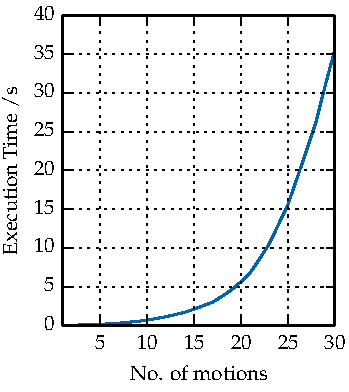
\includegraphics{gfx/ec/cec_swipl}}
\subfloat[TuProlog]
{\label{fig:cec_tupl}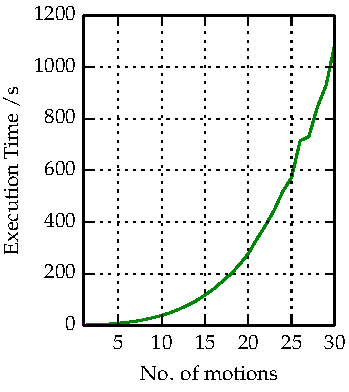
\includegraphics{gfx/ec/cec_tupl}}
\caption{Execution time of RONR using Cached Event Calculus with SWIProlog and
TuProlog engines}\label{fig:cec}
\end{figure}

\subsection{Integration with Java}

As we are working with a Java-based simulation tool, Presage2, we would like
to be able to interface with our electronic institution specification from
Java. This can be done either with a bridge between the Java application and a
Prolog interpreter, as offered by the JPL project
\footnote{http://www.swi-prolog.org/packages/jpl/java\_api/index.html}; or with a pure Java Prolog
engine. The former will offer comparable performance to the standalone Prolog
implementation, as the overhead of the communication between Java and Prolog
processes will be negligible (in relation to the runtime of the Prolog query).
The drawback of this method is portability: it requires a Prolog binary to be
available to the Java runtime.

Java Prolog engines offer a portable implementation which integrates natively
with Java code. tuProlog~\citep{Denti2005} is a lightweight Prolog
implementation in Java. We perform another performance test using this Prolog
engine to compare to those in the previous section.

We orchestrate the same testing scenario as before, with
identical narratives. The use of Java aids the automation of these tests, so
we run 10 repeats for each narrative. Additionally, runtime optimisation by
the Java Runtime Environment (JRE) means that the execution time will improve over
time, thus we exclude the first results, only taking results after the JRE has
`warmed-up'
\footnote{This `warm-up' refers to the dynamic, just-in-time compilation, and run-time optimisation performed by the JRE, which causes slower performance early in the program life-cycle~\citep{Blackburn2008}}. 
Timing is calculated using the Java built-in function
\texttt{System.nanoTime()}\footnote{http://docs.oracle.com/javase/7/docs/api/java/lang/System.html\#nanoTime()} 
which provides up-to nano second accuracy for timing tasks.

% TODO Results here
\autoref{fig:cec_tupl} shows the performance of the Cached Event Calculus running on
TuProlog. It shows that this engine is significantly slower than running the
same Prolog code in SWIProlog. However it scales slightly better, with the
performance going from 60 times slower with one motion,to 30 times at 30
motions.

%Despite this, given the significant runtime with relatively small
%numbers of actions, we do not see this as a viable approach.

\subsection{A rule-based implementation of EC axioms}

The Prolog implementations of the \ac{EC} provide deductive, abductive and
inductive reasoning capabilities. This allows for a broad range of tasks, such
as planning and monitoring. However, the cost of catering for all this tasks
in a single logic engine is shown in the computational complexity of seemingly
simple deductive tasks. If we wish to use an electronic institution, in a
simulation or application, purely for deductive tasks (to know what's true
when, given what has happened), then Prolog is not a very efficient solution.
We test this hypothesis by creating a proof-of-concept implementation of a
rule-based approach of the processing of \ac{EC} axioms, and testing its
performance with the same \ac{RONR} voting specification.

A purely deductive \ac{EC} implementation will only need to be able to query
for facts which can directly be inferred to be true. This will be either
whether a fluent \emph{holdsAt} a time \emph{t} (or what value it holds at
that t), whether a fluent is true \emph{initially}, whether an event happens
at a time t, or whether an event \emph{initiates} or \emph{terminates} a
fluent. We can specify this as a Java interface as shown in
\autoref{lst:iecquery}. This interface supports fluents with non-boolean
values, and also implicit inference of these values when passed a placeholder
object as the value.

\begin{java}[label=lst:iecquery,caption=Java interface for deductive queries on an EC Specification]
interface ECQuery {
	boolean holdsAt(Object fluent, int t);
	boolean holdsAt(Object fluent, Object value, int t);
	boolean happens(Object event, int t);
	boolean initially(Object fluent);
	boolean initially(Object fluent, Object value);
	boolean initiates(Object event, Object fluent, int t);
	boolean terminates(Object event, Object fluent, int t);
	boolean initiates(Object event, Object fluent, Object value, int t);
}
\end{java}

This interface uses the Java \texttt{Object} type for both fluent names,
fluent values and events. This gives maximum flexibility to the user, as all
types in Java extend from this base type. When querying, fluents and events
can be looked up using Java equality operators. These operators can be
overrided, such that more complex look-up functionality can be implemented.
This functionality is exploited in order to implement Prolog-style anonymous
and inferred variables in fluent names.

We also give a programmatic interface through which an \ac{EC} specification
can be given, shown in \autoref{lst:iecspec}. This interface also allows for
the assertion of facts at runtime, allowing the specification to manipulate
fluent values. The specification is given in terms of objects representing
rules, which define either what an event initiates, or whether a fluent holds.
An \emph{initiates} rule can define a fluent change by calling
\texttt{assertInitiates} which will update the value for that fluent at the
given time. \emph{HoldsAt} rules consist of a \texttt{Matcher} component, which
tests whether the rule matches a provided fluent, and a \texttt{Binder}, which
infers the value of the given fluent at a specified time.

\begin{java}[label=lst:iecspec,caption=Java interface for declaration of an EC specification]
interface ECSpecification {
	void initiates(InitiatesRule rule);
	void holdsAt(HoldsAt rule);
	void assertInitially(Object fluent);
	void assertInitially(Object fluent, Object value);
	void assertHappens(Object event, int t);
	void assertInitiates(Object event, Object fluent, Object value, int t);
}
\end{java}

In order to simplify translation of \ac{EC} specifications written in Prolog
we implement objects to represent predicates and tuples, including
\texttt{Matcher} implementations in order to perform dynamic matching of these
objects with anonymous and infered variables. For example we could match a
Prolog predicate \texttt{pow(V, vote(V,M,\_))}, inferring the values of
\texttt{V} and \texttt{M} in the process. Examples of both types of rule
specification are shown in \autoref{lst:initiates} and \autoref{lst:holdsAt}.
Note, this method achieves a one-to-one correspondance between \ac{EC} axioms
and rules. However, the verbose nature of Java results in a long, and
difficult to read specification.

\begin{java}[label=lst:initiates, caption={[Example of initiates rule]Example of initiates rule. Matchers are used to built a description of the event we wish to match. The matched arguments in this event are then used in the \emph{holdsAt} query to check whether the actor is empowered to perform the action. If the event and query are both valid we assert the change to the \emph{status} predicate.}]
// initiates( open_ballot(C,M), status(M)=voting(T), T ) :-
//     holdsAt( pow(C, open_ballot(C,M))=true, T ).
ec.initiates(new InitiatesRule() {
	Matcher C = new AnyStringMatcher();
	Matcher M = new AnyStringMatcher();
	Matcher open_ballot = new PredicateMatcher("open_ballot", C, M);

	public void apply(Object action, int t, SimpleEC ec) {
		if (open_ballot.matches(action)
				&& ec.holdsAt(new Predicate("pow", C.getLastMatch(),
						new Predicate("open_ballot", C.getLastMatch(),
								M.getLastMatch())), t)) {
			ec.assertInitiates(action,
					new Predicate("status", M.getLastMatch()),
					new Predicate("voting", t), t);
		}
	}
});
\end{java}

\begin{java}[label=lst:holdsAt,caption={[Example of \emph{holdsAt} rule]Example of \emph{holdsAt} rule. The \texttt{matches} function filters fluents which match the form we're looking for. If the fluent matches, \texttt{inferValue} determines the value based on the status of other fluents and using matched values from the specified fluent.}]
// holdsAt( pow(C, open_session(C,S))=true, T ) :-
//    holdsAt( sitting(S)=false, T ),
//    holdsAt( role_of(C,chair)=true, T ).
ec.holdsAt(new HoldsAt() {
	final MultiStringMatcher C = new MultiStringMatcher();
	final Matcher S = new AnyStringMatcher();
	final Matcher open_session = new PredicateMatcher("open_session",
			C, S);
	final Matcher pow_open_session = new PredicateMatcher("pow",
			C.master, open_session);

	public boolean matches(Object o) {
				return pow_open_session.matches(o);
			}

	public Object inferValue(Object fluent, int t, ECQuery ec) {
		return !ec.holdsAt(new Predicate("sitting", S.getLastMatch()), t)
				&& ec.holdsAt(new Predicate("role_of",
						C.getLastMatch(), "chair"), t);
	}
});
\end{java}

Our implementation of this rule-based \ac{EC} is a simple inference
engine. A fluent cache stores the values of strongly asserted fluents at each
discrete time point. Strongly asserted fluents are ones which have been
explicity set with \texttt{assertInitially} or \texttt{assertInitiates}. When
an event is asserted at time $\mathit{t1}$ it invalidates the cache for $t >= \mathit{t1}$. All
events after and including those at $\mathit{t1}$ are then processed. An event is
processed by triggering all initiates rules with the event and time pair. The
fluent cache is dynamically expanded for new timesteps by simply copying the
cache for the previous time. Deductive queries are handled by firstly looking
for a matching fluent in the cache. If non is found, each \texttt{Matcher} in
the set of \emph{HoldsAt} rules is checked to find a candidate rule to infer the value
with. If one is found, we use the \texttt{Binder} to return, or check the value
of the fluent.

We can translate the \ac{RONR} specification to run with this implementation,
and then again run our test-suite to determine performance. As before, we
perform 50 repeats of each narrative and allow for the Java Runtime
Environment to `warm-up' before collecting results. The results are shown in \autoref{fig:rulec}.

\begin{figure}
\centering
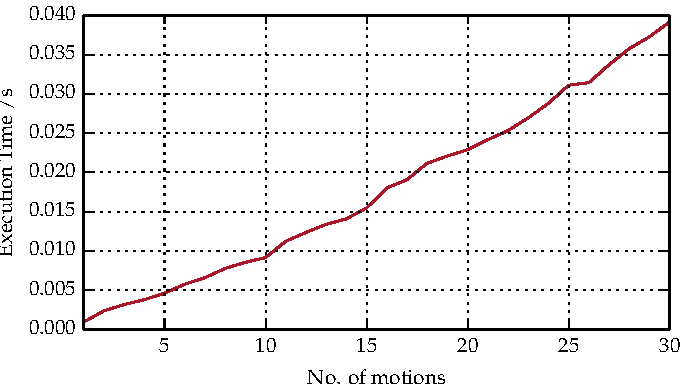
\includegraphics{gfx/ec/rulebased}
\caption{Execution time of RONR using a rule-based EC implementation.}\label{fig:rulec}
\end{figure}


Note that this runtime is several orders of magnitude faster than any other
implementation tested in this section. From this result we can draw the
conclusion that, if only deduction is required, a rule-based implementation of
the \ac{EC} will scale much better than with Prolog.

However, we note that this is a simple, and fairly naive implementation of a
rule-based approach to the \ac{EC}. It omits features such a forward-chaining,
which would be required to probably handle multiple actions per timestep. In
particular this implementation requires a verbose translation of the Prolog
specification, a process which is likely to introduce errors. The format of
these translated rules is fairly structured and uniform, therefore it would be
possible to write a compiler from \ac{EC} axioms to these programmatic rule
implementations. However, there already exist Java rule engines which have
declarative rule definitions, and employ much more robust and optimised 
rule-processing algorithms. We discuss how we can leverage these Production Rule
Engines in the next section.

An additional issue when using Prolog-like syntax for axioms is the
limitations of tuple- and predicate-based variables. This variable system is
readable and expressive with simple constructs, however lacks robust mechanisms to
reference other objects, and as the size and depth of nested tuples increases
readability is lost. This is in contrast to Java where we can have many member
variables in an object, and complex reference trees from these variables. This
shortcoming is highlighted in \ac{EC} specifications, where multiple different
fluents are used to describe different aspects of a single entity, while in
Java one would have a single object with multiple attributes.

\subsection{Summary of \acl{EC} Performance}

In summary, this section has outlined the issues with using direct prolog
implementations of the \ac{EC} when dealing with primarily deductive tasks,
and interfacing these with a Java runtime. Furthermore, by implementing a
simple version of rule-based deduction of fluents from translated \ac{EC}
axioms we observe an improvement in performance of several orders of
magnitude. Thus we propose that we can achieve a fast and robust deductive
\ac{EC} engine using a standard rule engine.

There is still ongoing work in implementing faster Prolog \ac{EC}
specifications, which haven't been tested here. RTEC~\citep{Artikis2012} for
example has been shown to achieve performance in event recognition tasks
comparable to that of rule-based approaches, using a rolling time window to
reduce the length of fluent history to store, and compiling axioms into
optimised forms. However, this approach requires specifications to be
translated into a special dialect of the \ac{EC}, and additional metadata to be
specified for events and fluents for the compiler's optimisation algorithm. 
This requires in depth knowledge of the optimisations and how to exploit them, 
which is a significant hurdle to the implementation of specifications.

The use of time windows has also been proposed by \citet{Carr2010} to speed up
the \ac{EC}. This method specifies a cut-off time point before which one can
no longer perform \emph{holdsAt} queries. In doing so the number of relevant
events can be reduced, and so, more linear scaling can be achieved. There is
then a trade-off to be made between the amount of history to be kept, and
query/event processing run time.

\section{A Rule-Engine Implementation of Event Calculus Specifications}

In the previous section we demonstrated both speed and scaling issues with
Prolog implementations of the \ac{EC}, and showed that for purely deductive
reasoning a rule-based approach is significantly faster. While specification
of an Electronic Institution in \ac{EC} is still worthwhile, particularly for
verification and the other non-deductive reasoning tasks, for runtime
deductive reasoning with large number of incoming events we advocate a 
rule-based implementation. Therefore, if we are specifying in \ac{EC}, but
implementing in a different paradigm we require a robust translation process
so that we can be confident of maintaining correctness.

In this section we present a method of translating \ac{EC} axioms into a
declarative rule form, using the language of a \acl{PRS} system, JBoss Drools.
We also present our implementation of a framework, and module library, 
Drools-EInst, to enable the use of specifications translated with this method within
a Java program, and the current set of modules implemented from various
\ac{EC} specifications. Finally, we give a runtime performance comparison
using the same \ac{RONR} example as in the previous section.

\subsection{JBoss Drools}

JBoss Drools\footnote{http://www.drools.org/} is a \ac{BRMS}, a software framework through which Knowledge
Representation and Reasoning can be done. The core component of this is a \ac{PRS}
which provides an ontology for knowledge representation and rules which the system
uses to reason with. This system is then fed data, through which it determines a
knowledge state. Drools' \ac{PRS} has a rule engine which employs hybrid reasoning,
enabling both forward-chaining and backward-chaining reasoning.

In a \ac{PRS}, `knowledge' is represented as rules. These rules specify a
condition which, when matched, causes a consequence. This matching is done
against a state, which is data expressed with the rule system's ontology. 

The Drools rule engine is implemented with an improved version of the Rete
algorithm (originally proposed by \citet{Forgy1982}). This algorithm optimises
the speed of pattern matching in the rule engine by employing a network of
nodes. Drools has developed various extensions to the original algorithm to
improve performance, properly integrate Java objects, and fuzzy reasoning\footnote{A full description of the algorithm is given in the software
documentation, available at \url{http://docs.jboss.org/drools/release/6.1.0.Final/drools-docs/html/HybridReasoningChapter.html}}.

The Drools \ac{PRS} then consists of the following at runtime:
\begin{itemize}
	\item Production Memory, which contains the production rules;
	\item Working Memory, which contains the state of the system, also called `facts';
	\item A Pattern Matcher, which matches production rules against facts or fact
	tuples;
	\item The Agenda, which is the set of matched rules paired with matched fact
	tuples. When a rule and set of facts are added to the agenda it is called an `activation'.
\end{itemize}

With the former two being specified and initialised by the user, the latter two
are part of the rule-engine implementation.

Drools allows the user to control the execution of rules through a \texttt{fireAllRules} method.
This procedure will start recursively executing the consequences of matched
rules until there are none remaining. Each consequence will cause insertion,
retraction or modification of facts in the working memory, which in turn may
cause matched rules to be added or removed from the agenda. Thus this enables
forward-chaining reasoning.

Rules are specified in a custom Drools rule language, which allows for
declarative rule specification with tight Java integration. Rules are written as
shown in \autoref{lst:droolsrule}. A `when' section describes the condition
to trigger the rule. This consists of object types with constraints which match
to facts. These conditional elements can be combined with various logical
operators to form a matching tuple. Furthermore, variables can be bound with the
unification operator (\texttt{:}), which can then be referred to in a later
conditional element, and/or in the consequence. The consequence of the rule,
specified in the `then' section, is written in Java, with some syntactic
shortcuts given for convenience. Namely, one can \texttt{insert}, \texttt{update}
and/or \texttt{retract} facts with shorthand functions.

\begin{drools}[label=lst:droolsrule,caption=Syntax of a Drools rule.]
rule "Rule name"
when
	Pattern1(constraints...)
	Pattern2()
then
	insert(...)
end
\end{drools}

The rule-engine also supports what is called `logical' insertion of a fact. If a
fact is inserted `logically' then its truth is dependant on the truth of the
`when' clause that led to its assertion. This means that the fact will be
automatically retracted if this conditional becomes false.

Backward-chaining reasoning and state checking is done through \emph{queries}.
These are written in the same syntax as when conditions and are able to unify
matching fact tuples, or sets of fact tuples using full or partial input data. 

Drools also has support for Complex Event Processing. This extension allows for
special facts, called events. These events are attached with temporal properties
to enable the use of temporal constraints in rules. Furthermore the rule engine
can manage the lifecycle of the event objects, so events which can no longer be
matched by a rule can be removed from the working memory to save space.

\subsection{Electronic Institution Implementation in JBoss Drools}

Drools offers a rich syntax for the specification of institutional rules.
Coupled with the event processing tools it enables logical and temporal
constraints for rules, coupled with native integration of Java objects.
Furthermore, it allows multiple state changes as a consequence of a rule, unlike
the \ac{EC} in which multiple clauses must be written to update multiple
fluents, even if they are caused by the same event. Therefore, we consider it as
a viable platform for the construction of a Electronic Institution engine.

However, there are several main design challenges to overcome to be able to transfer
\ac{EC} specifications into Drools:
\begin{enumerate}
\item The \ac{EC} allows reasoning of the state of the system in the past. This is
done either by holding a cache of all the previous states of fluents, or being
able to re-calculate this state from first principles. Drools' working memory
has no concept of \emph{when} a fact is true, only that the fact's current
state is true at the present point in time.
\item Facts in Drools must be concrete. Unlike in the \ac{EC}, where fluents can
hold with anonymous or fuzzily defined values, in Drools every fact is an
instantiated object. By default this object will then only match a object with
the same values in all of its member variables. Particularly when dealing with
institutionalised power it is important to be able to specify that an agent is
empowered to perform a particular \emph{type} of action, but with some specifics
omitted.
\item Nested fact matching. Drools does not support nesting of pattern within
another pattern. For this kind of matching we require separate patterns and a
constraint to show that the first match should be nested in the second pattern.
\item Queries cannot be overloaded. In the \ac{EC} queries such as \texttt{holdsAt}
are often defined multiple times for different input fluents. In Drools we would
only be able to have a single query definition which must handle all cases.
\end{enumerate}

\citet{Bragaglia2012} overcome these issues by requiring that a specification
only consists of \emph{initiates} clauses, defined in Java code. These clauses
are then compiled into Drools rules which assert the internal events
\texttt{Clip} and \texttt{Declip}. Validity intervals can then be calculated
in order to determine when fluents are true. This implementation therefore only
utilises Drools' rule language for the specification of \ac{EC} axioms, and the
actual domain specification must be done in Java code.

% The semantics of Drools make it very difficult to overcome the first issue
% efficiently, while maintaining simple, readable rules. Several issues conflict
% to 
% \begin{enumerate}
% \item A query or fact could be used to represent the value of a fluent at a time
% \texttt{\$t}: \texttt{HoldsAt(\$f:fluent, t==\$t)}. 
% \item As we cannot match this fluent within this conditional we must add a
% second clause to match the fluent: \texttt{Fluent(this==\$f, constraints...)}
% \item However, matching a fact like this require that it is asserted in the
% working memory. Therefore, all fluent values, past and present, must be inserted
% into the working memory.
% \item As the working memory is a \emph{set} of objects, all fluents cannot be
% \emph{equal} (as defined by the Java \texttt{equals} function). Therefore 
% \end{enumerate}
% However, there are a two limitations of Drools' features which require a
% trade-off to be made between the readability of rules, and the features we can
% achieve in the engine.

For these reasons we take a different approach. Rather than implementing \ac{EC}
axioms in Drools, we instead follow a process to translate \ac{EC}
specifications to work within a Drools workflow. Therefore instead of \emph{initiaties}
and \emph{holdsAt} axioms, we simply write Drools rules, and follow Drools
conventions.

The working memory holds the current state of fluents. We assume that events
are in order, so the state of the system when the event occurs should be
relevant to the event processing. When historical state is required extra
rules can be written to store this. This approach has the following advantages:
\begin{itemize}
\item We only store historical information about fluents when it is needed,
reducing space complexity of the engine.
\item We no longer need to nest fluents in queries of facts to indicate
their validity interval, preventing the need for nested fact matching for this
use.
\item \emph{holdsAt} queries are replaced with simple conditionals for the
fluents themselves, so we no longer need to overload queries.
\end{itemize}

Therefore we have addressed the first and fourth design challenges, and one use-case
of the third. 

The remaining issue is that of enabling the loose matching of
actions. The particular use-case here is granting institutionalised power,
permission or obligation to perform an action, where we wish to specify a range
of possible actions. We can create a fact to represent the agent-action tuple in
an object. For example we have a class \texttt{Pow} with \texttt{actor} and
\texttt{action} fields. A naive usage of this power would be to just check that
an event matches this action:

\begin{droolsinline}
$act : Action($a : actor)
Pow(actor == $a, action == $act)
\end{droolsinline}

However, this approach will only work in a very narrow range of cases.
Firstly, we must explicitly specify all attributes of the action which the
agent is empowered to do. In cases where there are several possible valid
actions (for example voting) we must enumerate each possible action.
Furthermore, it is possible in some cases that the set of possible actions is
infinite. Thus, this method is inappropriate for the task.

We enable ranges of actions to be specified by implementing a \texttt{matches}
method in \texttt{Pow}. This method checks whether a given action \emph{matches}
the range of actions specified in this \texttt{Pow} object. This range of
actions is defined by an object of the desired action type which may have some
fields set to \texttt{null}. The \emph{matches} method returns true if and only
if both actions are of the same type, and for each non-null field the values are
equal. Note, as this equality is defined on a per-object basis, it can be
overridden to provide nested dynamic matching. This method allows simple
specification of a range of allowed actions, and simple use of institutionalised
power in rules. To amend the previous example:

\begin{droolsinline}
$act : Action($a : actor)
Pow(actor == $a, action.matches($act))
\end{droolsinline}

\subsection{Translation of EC Electronic Institution Specifications}

With the design groundwork in place we now demonstrate how \ac{EC}
specifications can be translated into Drools. We present this translations as a
set of steps to undertake, and illustrate these steps with examples of the
translation of the original \ac{RONR} specification.

\subsubsection*{Declaration of events}

Events should be declared as Java objects, extending the provided base
\texttt{Action} class. This base class allows the engine to distinguish
actions from fluents, and attach time and other metadata to the action. The
event object should be immutable, when possible, as it is a constant. \autoref{lst:ClOpenSession}
shows the \emph{open\_session} event from \ac{RONR} as a Java object. 

\begin{java}[label=lst:ClOpenSession,caption=OpenSession action as a Java object]
public class OpenSession extends Action {

	final String name;
	
	public OpenSession(Actor actor, Institution inst, String sessionName) {
		super(actor, inst);
		this.name = sessionName;
	}
}
\end{java}

\subsubsection*{Representation of fluents}

We can simplify the state representations of electronic institutions by collected
related fluents into objects. For example, in \ac{RONR} there are separate
fluents for the status of a motion and the number of votes each way on it.
Furthermore there is no fluent expressing the link between a motion and the
session it is occurring in. We can easily encapsulate all this information in a
\texttt{Motion} object. 

The \ac{EC} specification also uses string identifiers to reference entities
such as motions and sessions. In Java and Drools we can directly reference other
objects, which is a much more robust form of linking, and prevents possible key
clashes or ambiguities.

\subsubsection*{Translation of Initiates clauses}

An \emph{initiates} clause is written in Prolog in the form:

\begin{prologinline}
initiates( event, fluent=value, T ) :-
	holdsAt( condition1, T ),
	...
	holdsAt( conditionN, T ).
\end{prologinline}

This can be translated into Drools roughly as follows:
\begin{droolsinline}
rule "Initiates example"
when
	Event(constraints...)
	$fluent : Fluent(condition1)
	...
	OtherFluent(conditionN)
then
	modify($fluent) {
		setValue(value)
	}
end
\end{droolsinline}

The first line of the Drools rule matches an event when it occurs. As well as
constraints on the event we can also bind attributes of the event to variables
to use later in the \emph{when} or \emph{then} clauses. The subsequent lines
in the \emph{when} clause perform two purposes: Firstly they test for fluents
matching the given constraints at the current time. Secondly, they gather any
other information from fluents, including the fluent to be modified itself,
which are needed in the \emph{then} clause. The \emph{then} clause then
performs the desired change in value to the fluent. Note that in Drools we can
perform multiple modifications to the working memory during a \emph{then}
clause, so it some cases, where there are multiple fluents to be updated from
a single event with the same conditions, we can reduce several \ac{EC} axioms
into one Drools rule.

With \emph{initiates} rules, we must also consider when a rule be activated. A
change to any object in the set of conditions on a rule may cause it to be
activated. While, with such a rule, we only want an activation to occur when the
event is inserted and the conditions are true, if the event remains in the
working memory it may cause an activation later if the conditions become true.
Therefore we require a mechanism to falsify the event condition after initial
processing.

We provide two such mechanisms, which work for different use-cases. Firstly, a
\texttt{valid} attribute is attached to actions. This attribute is false
initially, and should be set to true when the action is processed by a rule.
This means that the rule can be prevented from re-activated for this event by
using a \texttt{valid==false} constraint. The engine will then clean up any
invalid actions each timestep to prevent activations. The second method uses a
fact \texttt{T} which gives the most recent timestep. This can then be
compared to the attribute \texttt{t} of the action to ensure that the clause
can only be activated in this timestep. These two methods are shown below:

\begin{droolsinline}
rule "Validity check"
when
	$e : Event(valid == false)
	// conditions...
then
	modify($e) {
		setValid(true) // rule can no longer be triggered for this event
	}
	// other changes...
end
rule "Timestep check"
	T($t : t)
	Event(t == $t)
	// conditions...
then
	// other changes...
end
\end{droolsinline}

To illustrate this process in practice, we give two examples from \ac{RONR}.
\autoref{lst:ronrinitiates} shows the original Prolog and the translated
Drools rules. In this case, there are two rules to be triggered off the same
action, so we cannot use the \emph{valid} attribute for both. As the second
rule will trigger between zero and several times, depending on how many agents
qualified for the `seconder' role, this uses \texttt{T} for activation
control. In this second rule we can also avoid checking the institutional
power again, as it is implicitly true by virtue of the action being
\emph{valid}. Note also the additional clause in this rule to retrieve the
\texttt{RoleOf} fluent we wish to retract.

\begin{drools}[label=lst:ronrinitiates,caption={[Example of translated RONR initiates clauses.]Example of translated RONR initiates clauses. Original Prolog specification is shown in the comment above each rule.}]
//	initiates( second(B,M), status(M)=seconded, T ) :-
//		holdsAt( pow(B, second(B,M))=true, T ).
rule "Second"
	when
		$sec : Second($b : actor, $m : motion, valid == false)
		Pow(actor == $b, this.matches($sec))
	then
		modify($m) {
			setStatus(Motion.Status.Seconded);
		}
		modify($sec) {
			setValid(true);
		}
end

//	initiates( second(B1,M), role_of(B2,seconder)=false, T ) :-
//		holdsAt( pow(B1, second(B1,M))=true, T ),
//		holdsAt( qualifies(B2,seconder)=true, T ).
rule "Unassign seconders"
	when
		T($t : t)
		Second($i : inst, valid == true, t == $t)
		Qualifies($a : actor, role == "seconder")
		$r : RoleOf(actor == $a, $role == "seconder", inst == $i)
	then
		retract($r);
end
\end{drools}

\subsubsection*{Translation of HoldsAt clauses}

\emph{HoldsAt} clauses in the ac{EC} state that a fluent is true when certain
conditions are satisfied. They can be written in Prolog as follows:

\begin{prologinline}
holdsAt( fluent=value, T) :-
	holdsAt( condition1, T),
	holdsAt( conditionN, T).
\end{prologinline}

These can also be simply implemented with rules in Drools. As the resulting fluent is only true when the conditions hold, we use the \texttt{insertLogical} feature of Drools. This ensures that if the conditions no longer hold, the fact will be automatically retracted. The translated clause is therefore as follows:

\begin{droolsinline}
rule "Holdsat example"
when
	Fluent(condition1)
	...
	OtherFluent(conditionN)
then
	insertLogical(new Fluent(value));
end
\end{droolsinline}

\autoref{lst:droolsholdsat} shows an example rule from ac{RONR}. Each
condition from Prolog becomes a Drools condition, and the bound variables are
used to construct the relevant institutionalised power.

\begin{drools}[label=lst:droolsholdsat,caption={[Example of a translated RONR holdsAt clause.]Example of a translated RONR holdsAt clause. Original Prolog specification is shown in the comment the rule.}]
//	holdsAt( pow(B, second(B,M))=true, T ) :-
//		holdsAt( status(M)=proposed, T ),
//		holdsAt( role_of(B,seconder)=true, T ).
rule "Pow second motion"
	when
		RoleOf($b : actor, $i : inst, role == "seconder")
		$m : Motion(status == Motion.Status.Proposed)
	then
		insertLogical(new Pow($b, new Second($b, $m)));
end
\end{drools}

\subsubsection*{Limitations of anonymous variables}

We described our method of enabling matching of actions with anonymous
variables in Drools. This method imitates the underscore operator in Prolog,
allowing any value to match that field. However, in some cases we wish to
specify that a field may be any value \emph{except} ones within a certain set.
This cannot currently be implemented, however it can be overcome with a simple
workaround.

Returning to the \ac{RONR} example, we can see a case where this problem arise in the following clause:

\begin{prologinline}
holdsAt( pow(C, open_session(C,S))=true, T ) :-
	holdsAt( sitting(S)=false, T ),
	holdsAt( role_of(C,chair)=true, T ).
\end{prologinline}

This specifies that an agent is empowered to perform the \emph{open\_session}
action for any session which is \emph{not} sitting (\ie an infinite set of
actions, minus a finite set of exceptions). In Drools we can only specify that
the agent is empowered to open \emph{any} session. Therefore, in order to
maintain this condition, and so that we do not process an action incorrectly,
we can move this condition to the rule which processes the action, as shown in
\autoref{lst:droolsanon}. The first rule allows for the agent in the `chair'
role to open a session with any name by setting that field to null. The check
for a conflicting session is then done in the second rule, once the action has
been performed.

\begin{drools}[label=lst:droolsanon,caption=Drools translation of RONR open session.]
rule "Pow open session"
	when
		RoleOf($c : actor, $i : inst, role == "chair")
	then
		insertLogical(new Pow($c, new OpenSession($c, $i, null)));
end

rule "Open Session"
	when
		$open : OpenSession($a : actor, $i : inst, $name : name, $t : t, valid == false)
		Pow(actor == $a, this.matches($open))
		not(exists(Session(inst == $i, name == $name, sitting == true)))
	then
		insert(new Session($i,  $name, true));
		modify($open) {
			setValid(true);
		}
end
\end{drools}

This approach is not ideal, as it could lead to an agent thinking it has power to do something when it does not. However, this is a limitation of the Drools rule language. For situations when this feature is critical, it may be possible to assert a negated power, \ie that the agent explicitly does not have the power to do an action. Using a query, this could be given precedence over the original \emph{Pow}, such that $\mathtt{power(Ag,Act) \leftarrow \mathtt{Pow(Ag,Act)} \land \lnot \mathtt{NotPow(Ag,Act)}}$. However, we have not yet implemented or tested such a feature, and it is left for future work.

\subsection{Drools-EInst}

We package together the tools and workflow described into a Java library,
called Drools-EInst. This library allows for the implementation of
specifications as modules. These modules consist of Drools rule files, which
implement a specification, and a Java \ac{API} for this specification. The
latter provides a high level interface to the state of the institution, as
well as methods to add or remove objects to the working memory from Java code.
These \ac{API}s act as the query and manipulation component of the Electronic
Institution.

We have implemented six modules from \ac{EC} specifications:

\begin{itemize}
\item Institutionalised Power -- Our implementation of institutionalised power, as has been used above. This enables powers, permissions and obligations to be specified for agents. Queries can then be done to check what power exists for agents. Additionally, we use a Drools feature called `LiveQuery' to allow for immediate notification when certain powers become true or false.
\item Access Control -- Assigns \texttt{RoleOf} facts according to the protocol from \citet{Pitt2012b}. This includes multiple role assignment methods.
\item Micro Payments -- A simple implementation of micro-payments within an institution.
\item Provision and Appropriation -- Manages provision and appropriation of heterogeneous resources to a pool, as set out in \autoref{sec:formalchar}. Enables the creation of multiple \emph{pools} which can specify certain types of resource which can be provisioned to them. Agents can request resources from the pool and appropriate them. Additionally allows for retraction/removal of resources. Power to do these actions is role-based, using the Access Control module for this.
\item \ac{RONR} -- The \ac{RONR} specification as given in \autoref{sec:ronrcode}.
\item Voting -- A more general voting protocol which enables multiple different vote types and winner determination methods.
\end{itemize}

Each module is thoroughly unit tested to ensure that the rules are functioning
correctly. This is done by running various narratives and then testing the
fluents match expected values.

\subsection{Performance Evaluation}

To compare the performance of the Drools-EInst engine to those tested in
\autoref{sec:ecperf} we run the same experiment again with our \ac{RONR}
implementation. We extend the test to 100 motions and compare the performance
to that of our simple rule-based \ac{EC} implementation. The results are shown
in \autoref{fig:droolsperf}. We see that the performance is several times
slower than this benchmark, but this is to be expected when going from a hard-coded
implementation to a dynamic rule engine with forward and backward
chaining. However, the performance hit is negligible when compared to the
Prolog implementations, and for longer narrative the performance gap to the
benchmark reduces.

\begin{figure}
\centering
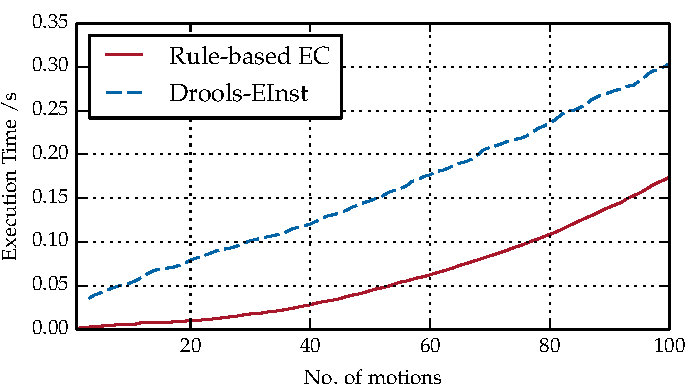
\includegraphics{gfx/ec/droolsvsrules}
\caption{Execution time of RONR using Drools-EInst implementation.}\label{fig:droolsperf}
\end{figure}

\subsection{Correctness of Specification Translation}

In this section we have presented a method of translating \ac{EC}
specifications in to Drools ones. Having performed this translation we want to
verify that the two specifications we have now are equivalent, that the
translation is provably \emph{correct}.

The deductive portion of the \ac{EC} can be characterised as a function which
maps a state (being a set of fluents), and a narrative (a set of actions) to a
new state. Similarly, we use Drools to do this same mapping from a state in
the rule-engine and a set of actions to a new state. Therefore a proof of
correctness must proof the equivalence of these two functions.
However, there are significant hurdles to such a proof:

Firstly, our translation process may cause some changes to the representation
of state and fluents. We change some fluents in order to take advantage of the
richer state representations possible in Java, and to better match the Drools
workflow. This means that we have an additional translation, from \ac{EC}
state and action representations, to those for Drools.

Secondly, the way we handle past values of fluents in the translation is
incompatible with the \ac{EC} method, therefore the new state generated by the
Drools implementation may only store a subset of past fluents, and therefore
not be equivalent anyway.

% Finally, while the \ac{EC} is a logical specification, and as such has well defined and provable properties, Drools is not so well defined and its algorithms are not fully formally defined. Therefore a proof would have to make significant assumptions about the correctness of 

This second issue would prevent full correctness being proved, but we may wish
to instead prove that the state concerning the latest time point is
equivalent. We do not yet have such a proof, and we leave this for future work.

However, instead of attempting to prove equivalence for all possible inputs,
we can instead test a subset thereof with unit testing. Using the same
framework as we did for benchmarking we can test a series of input state and
narratives in both specifications, and compare the output states between
\ac{EC} and with translated Drools rules. These input combinations can be
chosen to test each rule in isolation, and combined, and thus give a high
level of confidence in the correctness of the translation. This method is used
for all specifications implemented in Drools-EInst.

\section{Summary}

In this chapter we have investigated the operationalisation of electronic
institutions for specification of procedure and institutionalised power in
open agent systems. Existing methods, based on logics and action languages,
are rich in reasoning capabilities and expressive, however implementations
suffer from poor performance and scalability. Therefore, we advocate an
approach whereby such representations are still used for specification, but
for operationalisation a translation to production rules is made, allowing for
significantly faster event processing while maintaining expressiveness. We demonstrate this approach by
describing the translation of \ac{EC} axioms into rules for the Drools rule
engine, and the implementation of the Drools-EInst library for the processing
of institutional actions.

This approach is similar to that of \citet{Arcos2005} and
\citet{Aldewereld2006} in that logic-based specifications are translated into
faster constraint or rule specifications, however our method maintains a much
closer correspondence between logic and rule specifications. There is a 
one-to-one correspondence between \ac{EC} axioms and Drools rules, with each
\ac{EC} query becoming a single Drools condition. We believe this relation is
apparent when comparing between the specifications.

The cost of this performance improvement from \ac{EC} to Drools is the loss of
abductive and inductive reasoning over the specification, and the loss of the
cache of past values of fluents. As the implementation using rules is
primarily aimed at speeding up deductive at the cost of abduction and
induction this first loss is expected. The second is mitigated by the fact
that with Drools we can still explicitly store fluents describing historical
states, and therefore keep history in a more efficient manner.

Currently there are only a small number of modules implemented in the 
Drools-EInst library. We expect this to increase as it is used by more simulations
and applications. The modularity of the library's design enables it to be used
for rapid development and prototyping of Electronic Institutions. A user can
easily test various different module permutations, as well as rich
configuration options provided by each module itself. Thus, this library can
be seen as a toolkit for deploying Electronic Institutions into socio-technical 
systems.

% EC: 
% Combination of protocols (but slow)~\citep{Carr2012}. 
% Floor control~
% Provision and appropriation systems~\citep{Pitt2012}. 
% Voting protocols~\citep{Pitt2005a}. 
% Institutionalised consensus~\citep{Sanderson2012}. 
% Resource sharing~\citep{Artikis2005}.
% Monitoring and sanctioning~\citep{Pitt2012c}. 

% Argumentation Protocol (in C+)~\citep{Artikis2003}.

% Norms as rules with JESS~\citep{Garcia-Camino2005}.

% Constraints~\citep{Aldewereld2007}.

% Comparison EC to C+ Artikis2009 specifying norm-governed comp socieities

% Languages:
% InstAL
% C+ Giunchiglia2004
% EC
% AMELI